\documentclass[12pt,a4paper,oneside,english,spanish]{book}
\usepackage[a4paper, margin=1in]{geometry}
\usepackage[T1]{fontenc}
\usepackage{helvet}
\renewcommand{\familydefault}{\sfdefault}
\usepackage[utf8]{inputenc}
\usepackage[spanish]{babel}
\usepackage[document]{ragged2e}
\usepackage{graphicx}
\usepackage{longtable}
\usepackage{multirow} 
\usepackage{xcolor, colortbl}
\usepackage{hyperref}
\usepackage{comment}
\usepackage{array}
\usepackage{booktabs}
\usepackage{bigstrut}
\usepackage{float}
\usepackage{longtable}
\usepackage{pdfpages}
\usepackage[spanish]{babel}
\usepackage{biblatex}
\usepackage{csquotes}
\usepackage[acronym]{glossaries}
\makeglossaries
%%\usepackage{datetime}
%%\usepackage{mfirstuc}
%% PARA ROTAR TABLAS o PÁGINAS
\usepackage{lscape}

%%PARA DIAGRAMAS DE GANTT
%%\usepackage{tikz}
\usepackage{pgfgantt}
\usepackage{xcolor}

%%%%%%%%%%%%%%%%%%PAGE SETTINGS%%%%%%%%%%%%%%%%%%%%%%
\graphicspath{{img/}}
\addbibresource{bibliography.bib}

\definecolor{groupblue}{RGB}{51, 153, 255}
% Define the barblue color
\definecolor{barblue}{RGB}{0, 64, 128}
\definecolor{linkred}{RGB}{165,0,33}

%%Color para las tablas
%%\usepackage[table]{xcolor}% http://ctan.org/pkg/xcolor

%%--USAR ARCHIVO .BIB
%\usepackage{chicago}


\title{Monografía}
\author{}
\date{\today}
\setcounter{tocdepth}{3} 

\begin{document}

    \pagenumbering{gobble} 
    \renewcommand{\refname}{}
    \renewcommand{\tablename}{Tabla}


    %%--------------- PORTADA ------------------
    \begin{center}
    {\textbf{Propuesta de un mecanismo dinámico que permita contrarrestar el efecto de FWM en una red MLR-PON }}\\
    \vfill

    
\includegraphics[scale=0.7]{img/logo-unicauca.png} \\
    \vfill

    \textit{Monografía para optar por el título de Ingeniería Electrónica y Telecomunicaciones}\\
    Modalidad Trabajo de Investigación\\
    \vfill

    Santiago Sánchez Echavarría\\
    Andrés Felipe Diago Matta\\
    
    \vfill
    \textbf{Tutores:}\\
    Phd. Jose Giovanny López Perafán \\
    Phd. Carlos Andres Martos Ojeda \\
    
    \vfill
    Universidad del Cauca\\
    Facultad de Ingeniería en Electrónica y Telecomunicaciones\\
    Programa de Ingeniería en Electrónica y Telecomunicaciones\\
    Grupo de investigación de Nuevas Tecnologías en Telecomunicaciones - GNTT\\
    %Popayán, Cauca\\
    %Noviembre de 2023\\
    \date{\today}
    Popayán, \today
\end{center} 

        
    \newpage
    \renewcommand{\contentsname}{\centering TABLA DE CONTENIDO}
    \vfill
    \tableofcontents
    \cleardoublepage 

    \renewcommand{\listtablename}{\centering LISTA DE TABLAS}
    \listoftables
    \cleardoublepage 

    % lista de figuras
    \renewcommand{\listfigurename}{\centering LISTA DE FIGURAS}
    \listoffigures
    \cleardoublepage 

    %lista de acrónimos
    \newacronym{ai}{AI}{Artificial Intelligence}
\newacronym{ml}{ML}{Machine Learning}
\newacronym{tic}{TIC}{Tecnologías de la Información y de las Comunicaciones}


\begin{table}[h]
    \begin{tabular}{lcl}
        CNPq & – & Conselho Nacional de Desenvolvimento Científico e Tecnológico \\
        DS & – & Desenvolvimento Sustentável \\
        ITV & – & Instituto Tecnológico Vale \\
        MI & – & Mineração \\
        UFOP & – & Universidade Federal de Ouro Preto
    \end{tabular}
\end{table}

% OBSERVACIÓN:
% Incluir en orden alfabética
    \cleardoublepage 
    \printglossary[type=\acronymtype, title=\centering LISTA DE ACRÓNIMOS]


    \newpage
    % Restore page numbering after the pages without numbering
    \pagenumbering{arabic}

    \setcounter{page}{1}

\chapter{Introduction}
\label{chap1:introduction}

\begin{center}
    \item \section{PLANTEAMIENTO DEL PROBLEMA}
\end{center}


\justify %%justificar los párrafos

\vfill %espaciar los párrafos

%---revisar articulo 20, en lista primera búsqueda

En los últimos años ha tenido lugar un crecimiento del uso de las \gls{tic}. Esto ha provocado un gran incremento en el interés de las empresas por estar online y prestar sus servicios a través de plataformas digitales, actualizando sus herramientas de trabajo y digitalizando al máximo sus medios de producción. Este proceso de digitalización se ha visto potenciado por la proliferación de los servicios de almacenamiento y gestión en la nube, así como por la proliferación de dispositivos móviles inteligentes de bajo coste \cite{PedroRuiz}. 

Por esta razón, es importante abordar el tema de la seguridad, ya que la sociedad actual usa un gran número de aplicaciones, desde la banca en línea y aplicaciones de trabajo remoto hasta el entretenimiento personal y el comercio electrónico. Es por esto que, las aplicaciones se convierten el objetivo principal de los atacantes, que se aprovechan de las vulnerabilidades como los fallos de diseño, así como de las debilidades de las API, el código abierto, los widgets de terceros y el control de acceso, buscando acceder a bases de datos, servidores y otros datos sensibles. Si se logra la exposición de datos sensibles, es posible lanzar ataques de referencia u otras formas de fraude en línea.

Los atacantes digitales tienen la ventaja de contar con el  alcance y anonimato de quien los propicia, por lo que significa un gran reto para cualquier organización. Como prácticas de seguridad habituales se tiene el cambio de contraseñas, prohibir acceso a dispositivos y hacer una constante actualización de software. Pero esto no implica que la seguridad de las aplicaciones sea un factor que siempre se considere, siendo así un elemento por lo general ignorado y vulnerable. Esto genera una alta probabilidad de enfrentarse a amenazas que se generan por fallos del sistema a raíz de una inadecuada codificación, servidores mal configurados y un mal diseño en la aplicación.


Este trabajo de grado se va a desarrollar para la empresa WIZIT MIND BLOWING SOLUTIONS S.A.S, la cual es una empresa que se especializa en crear soluciones tecnológicas a la medida para sus clientes. El portafolio de servicios que ofrece, se encuentran soluciones en desarrollo de software, ciencia de datos, servicios en la nube, consultoría digital, entre otras líneas de negocio. Dentro de las soluciones que tienen una relación con plataformas tecnológicas, digitalización de procesos y software que está en la web, se utiliza entre otras tecnologías Node.js, que es una plataforma de desarrollo muy popular para aplicaciones web, y con su creciente adopción, la seguridad de las aplicaciones desarrolladas en Node.js se ha convertido en una preocupación crítica. 


Con lo mencionado anteriormente, este trabajo tiene como propósito la definición de un esquema/proceso replicable para la validación de pre-requisitos técnicos puede ayudar a minimizar la presencia de vulnerabilidades en estas aplicaciones, permitiendo un análisis de las vulnerabilidades comunes en aplicaciones desarrolladas con Node.js y la identificación de los pre-requisitos técnicos necesarios para prevenirlas. También implica la definición de un proceso replicable para validar la presencia de estos pre-requisitos técnicos en las plataformas de la empresa.



%%norma iso27001 -> https://www.iso.org/standard/27001

    \chapter{CONCEPTOS Y TECNOLOGÍAS}
\label{chap2:conceptos}

Una vez definido el motivo y los objetivos del trabajo y antes de dar un enfoque
directamente sobre el problema, es necesario saber la situación actual del mismo.
Comprender el objetivo, las tecnologías y arquitecturas utilizadas, es esencial para conocer el contexto del problema. En este capítulo hablaremos sobre los conceptos principales que se van a tratar a lo largo del proyecto.



\subsection{Four Wave Mixing (FWM)}
La Mezcla de Cuatro Ondas (FWM, por sus siglas en inglés \textit{Four Wave Mixing}) es un fenómeno no lineal que se manifiesta en sistemas de fibra óptica. Este efecto surge cuando dos o más señales ópticas, con frecuencias centrales diferentes, coexisten y se propagan a lo largo de una misma fibra.

En condiciones normales, estas señales ópticas deberían viajar independientemente sin interactuar significativamente entre sí. Sin embargo, debido a las no linealidades inherentes a la fibra óptica, como la no linealidad Kerr, las señales pueden influenciarse mutuamente.

El proceso de FWM implica la generación de nuevas componentes de frecuencia en la señal óptica original. Específicamente, se generan sumas y diferencias de las frecuencias originales, dando lugar a componentes espectrales adicionales. Este fenómeno puede introducir interferencias indeseadas entre los canales de comunicación en sistemas de multiplexación por división de longitud de onda (WDM), afectando negativamente la calidad de la señal y, en última instancia, la integridad de la transmisión de datos.

La FWM se convierte en un desafío significativo, especialmente en entornos donde se utilizan múltiples canales con frecuencias cercanas, como en sistemas WDM con canales igualmente espaciados. La supresión efectiva de la FWM es esencial para garantizar un rendimiento óptimo en las redes ópticas y maximizar la capacidad del sistema.

En el contexto de este trabajo, la propuesta de un mecanismo dinámico para contrarrestar la FWM en una red MLR-PON busca abordar este desafío, utilizando estrategias como la asignación de canales desigualmente espaciados y algoritmos optimizados para mitigar los efectos perjudiciales de la FWM.


\subsection{Redes MLR-PON}
Una Red de Acceso de Largo Alcance con Múltiples Longitudes de Onda (MLR-PON, por sus siglas en inglés \textit{Long-Reach Multiple Wavelength Passive Optical Network}) es una variante evolucionada de la Red Óptica Pasiva (PON). A diferencia de las PON convencionales, las MLR-PON están específicamente diseñadas para proporcionar alcances extendidos, lo que las hace adecuadas para entornos donde se requiere cobertura en áreas geográficas más extensas.

Las redes MLR-PON logran este aumento en el alcance mediante el empleo de múltiples longitudes de onda en la transmisión de señales ópticas a través de la fibra. Cada longitud de onda puede considerarse como un canal independiente, lo que permite la transmisión simultánea de datos a diferentes velocidades y servicios.

Este enfoque de múltiples longitudes de onda no solo extiende el alcance de la red, sino que también proporciona una mayor flexibilidad y capacidad de ancho de banda. Además, las MLR-PON son compatibles con servicios de voz, datos y video, ofreciendo una solución integral para las demandas crecientes de conectividad en entornos residenciales y empresariales.

La implementación de MLR-PON se ha vuelto crucial para superar las limitaciones de distancia asociadas con las PON tradicionales, especialmente en áreas geográficas dispersas. En el contexto de este trabajo, la propuesta de un mecanismo dinámico para contrarrestar la Mezcla de Cuatro Ondas (FWM) se enfoca en optimizar el rendimiento de las MLR-PON, abordando los desafíos específicos asociados con la interferencia no lineal en este tipo de redes.


\subsection{Asignación de Canales Desigualmente Espaciados}
La asignación de canales desigualmente espaciados es una estrategia de gestión del espectro en sistemas de transmisión óptica, donde las longitudes de onda utilizadas para la transmisión no siguen una separación uniforme. En contraste con la asignación de canales igualmente espaciados, donde la distancia entre las longitudes de onda adyacentes es constante, la asignación desigual implica una distribución no uniforme de las longitudes de onda a lo largo del espectro óptico.

Esta técnica se utiliza para abordar problemas específicos relacionados con la interferencia y la diafonía en sistemas ópticos, especialmente en entornos de multiplexación por división de longitud de onda (WDM). La asignación desigual de canales puede optimizarse para minimizar la interferencia no lineal, como la Mezcla de Cuatro Ondas (FWM, por sus siglas en inglés \textit{Four Wave Mixing}), que puede ocurrir cuando las señales ópticas tienen intensidades significativas y se propagan simultáneamente en la fibra.

Esta estrategia permite adaptar la distribución de las longitudes de onda a las características específicas de la red óptica, teniendo en cuenta las propiedades de transmisión de la fibra y los efectos no lineales asociados. Al asignar desigualmente las longitudes de onda, se pueden evitar ciertos patrones que contribuyen a la interferencia no deseada, mejorando así el rendimiento del sistema.

En el contexto de este trabajo, la propuesta de un mecanismo dinámico para contrarrestar la FWM en una red MLR-PON se centra en la asignación de canales desigualmente espaciados como una estrategia clave para mitigar los efectos no lineales y mejorar la calidad de la transmisión en este tipo de arquitecturas.


\subsection{Reglas de Golomb}
Las reglas de Golomb, y su generalización, las reglas g-Golomb, son conjuntos de enteros positivos con propiedades específicas utilizadas en la asignación de canales en sistemas ópticos.

\subsection{Algoritmos para Asignación de Canales}
Existen diversos algoritmos para asignar canales en redes ópticas, algunos se centran en la optimización de la distancia entre canales.

\subsection{Simulación por Agentes}
El uso de técnicas de simulación por agentes permite modelar y simular el comportamiento dinámico de la red.

\subsection{Mecanismos Dinámicos}
Un mecanismo dinámico implica la capacidad de adaptarse y cambiar en respuesta a las condiciones cambiantes de la red.

\subsection{Efectos No Lineales en Fibra Óptica}
Además de la FWM, otros efectos no lineales como la dispersión y la atenuación deben considerarse al diseñar una red óptica.

    \begin{center}
    \item  \section{OBJETIVOS}
\end{center}

\subsection{Objetivo general}

Definir un esquema/proceso replicable para la validación de pre-requisitos técnicos que minimicen la presencia de vulnerabilidades en plataformas desarrolladas en la empresa WIZIT MIND BLOWING SOLUTIONS S.A.S con Node.js.

\subsection{Objetivos específicos}
\begin{itemize}
    \item Caracterizar y priorizar posibles vulnerabilidades que existen al desarrollar aplicaciones nodejs en conjunto con express.
    \item Generar recomendaciones para prevenir ataques a partir de vulnerabilidades en situaciones específicas\footnote{Manual de reglas/ checklist, en concordancia con la norma ISO 27001}.
    \item Desarrollar un piloto que aplique las reglas definidas.
    \item Evaluar la efectividad del esquema/proceso replicable propuesto en la prevención de vulnerabilidades en plataformas desarrolladas en la empresa con Node.js, a través de la aplicación piloto y la comparación de los resultados obtenidos antes y después de aplicar las reglas definidas.
\end{itemize}

%% RECOMENDACIONES: se recomienda incluir el aspecto de la evaluación de las reglas propuestas en uno de los objetivos
%% Buscar un propósito para el modelo que se va a definir, el objetivo que recomendaron añadir

%%PROPOSITO: es establecer un esquema/proceso replicable para la validación de pre-requisitos técnicos en el desarrollo de aplicaciones en la empresa con Node.js. Este modelo tiene como objetivo minimizar la presencia de vulnerabilidades en las plataformas desarrolladas, brindando un enfoque estructurado y sistemático para identificar y mitigar posibles vulnerabilidades.
%El modelo propuesto busca proporcionar pautas claras y específicas para el desarrollo seguro de aplicaciones con Node.js, teniendo en cuenta las mejores prácticas y consideraciones de seguridad. Además, busca caracterizar y priorizar las vulnerabilidades comunes asociadas al uso de Node.js y su integración con Express, permitiendo la generación de recomendaciones y reglas para prevenir ataques en situaciones específicas.

%% ¿como aplicar el manual o checklist?, es posible pre, o post a la entrega de un desarrollo, o en el proceso de desarrollo de un desarrollo
%% seria necesario familiarizar el manual o checklist para el equipo de desarrollo, para que se pueda aplicar 
    \begin{center}
\section{METODOLOGÍA, ACTIVIDADES Y CRONOGRAMA}
\end{center}

\subsection{METODOLOGÍA}
La metodología que se utilizará como referencia en el desarrollo del trabajo de grado en modalidad práctica profesional es la metodología del PMI. Este tipo de metodología proporciona un desarrollo del proyecto de manera gradual en la ejecución de los objetivos propuestos a través de procesos que se mencionan a continuación: Proceso de iniciación, Proceso de planificación, Proceso de ejecución, Proceso de supervisión y control, Proceso de cierre del proyecto.

\subsection{FASES Y ACTIVIDADES}
\begin{longtable}[htbp]{|p{4.055em}|p{11.22em}|p{20em}|}
  \caption{Fases y Actividades} \\
  \hline
  \multicolumn{1}{|c|}{\textbf{FASE}} & \textbf{NOMBRE} & \textbf{ACTIVIDADES} \bigstrut\\
  \hline
  \endfirsthead
  \multicolumn{3}{c}%
  {\tablename\ \thetable\ -- \textit{Fases y Actividades}} \\
  \hline
  \multicolumn{1}{|c|}{\textbf{FASE}} & \textbf{NOMBRE} & \textbf{ACTIVIDADES} \bigstrut\\
  \hline
  \endhead
  \hline
  \multicolumn{3}{r}{\textit{Continúa en la siguiente página}} \\
  \endfoot
  \hline
  \endlastfoot
  \multirow{4}{*}{\centering\textbf{I}} & Proceso de iniciación & 
  1. Recopilar información sobre prácticas de seguridad en la empresa WIZIT MIND BLOWING SOLUTIONS S.A.S, y sobre la norma ISO 27001: Realizar entrevistas o reuniones con representantes de la empresa para conocer las prácticas de seguridad actuales, los procedimientos implementados y las políticas establecidas. \newline{}
  2. Identificar los sistemas y aplicaciones desarrollados en Node.js: Obtener un inventario de las plataformas y aplicaciones desarrolladas en Node.js por la empresa, así como su importancia y criticidad. \newline{}
  3. Analizar las vulnerabilidades comunes en aplicaciones web con Node.js: Realizar una revisión de la literatura y recopilar información sobre las vulnerabilidades más frecuentes que afectan a las aplicaciones web desarrolladas en Node.js. \newline{}
  4. Definir el alcance y los objetivos específicos del proyecto: Asegurarse de que los objetivos establecidos anteriormente sean claros y alineados con las necesidades de la empresa WIZIT MIND BLOWING SOLUTIONS S.A.S. \bigstrut\\
  \hline
  \multirow{3}{*}{\centering\textbf{II}} & Proceso de Planificación & 
  5. Establecer el alcance del proceso, indicando qué aplicaciones y plataformas de la empresa estarán cubiertas por el esquema de seguridad en capas.\newline{}
  6. Identificar las capas de seguridad y las medidas correspondientes.\newline{}
  7. Establecer criterios de selección de tecnologías y herramientas disponibles para el desarrollo con Node.js. \bigstrut\\
  \hline
  \multirow{3}{*}{\centering\textbf{III}} & Proceso de Ejecución & 
  8. Implementar las capas de seguridad seleccionadas, con las medidas de seguridad correspondientes en cada capa.\newline{}
  9. Implementar las herramientas y tecnologías de seguridad elegidas durante la fase de planificación.\newline{}
  10. Elaborar documentación detallada que describa las medidas de seguridad implementadas en cada capa, para su correcta aplicación en la empresa WIZIT MIND BLOWING SOLUTIONS S.A.S. \bigstrut\\
  \hline
  \multirow{2}{*}{\centering\textbf{IV}} & Proceso de Supervisión & 
  11. Evaluar el estado de seguridad de las aplicaciones y verificar la efectividad de las medidas implementadas.\newline{}
  12. Documentar los hallazgos, identificar áreas de mejora y proponer acciones correctivas o preventivas. \bigstrut\\
  \hline
  \multirow{3}{*}{\centering\textbf{V}} & Proceso de Cierre del Proyecto & 
  13. Entrega de documentos (Documento final y archivos del modelo replicable).\newline{}
  14. Entrega del modelo de seguridad en capas a la empresa WIZIT MIND BLOWING SOLUTIONS S.A.S.\newline{}
  15. Preparación y realización de la sustentación. \bigstrut\\
  \hline
\end{longtable}


\begin{landscape}
  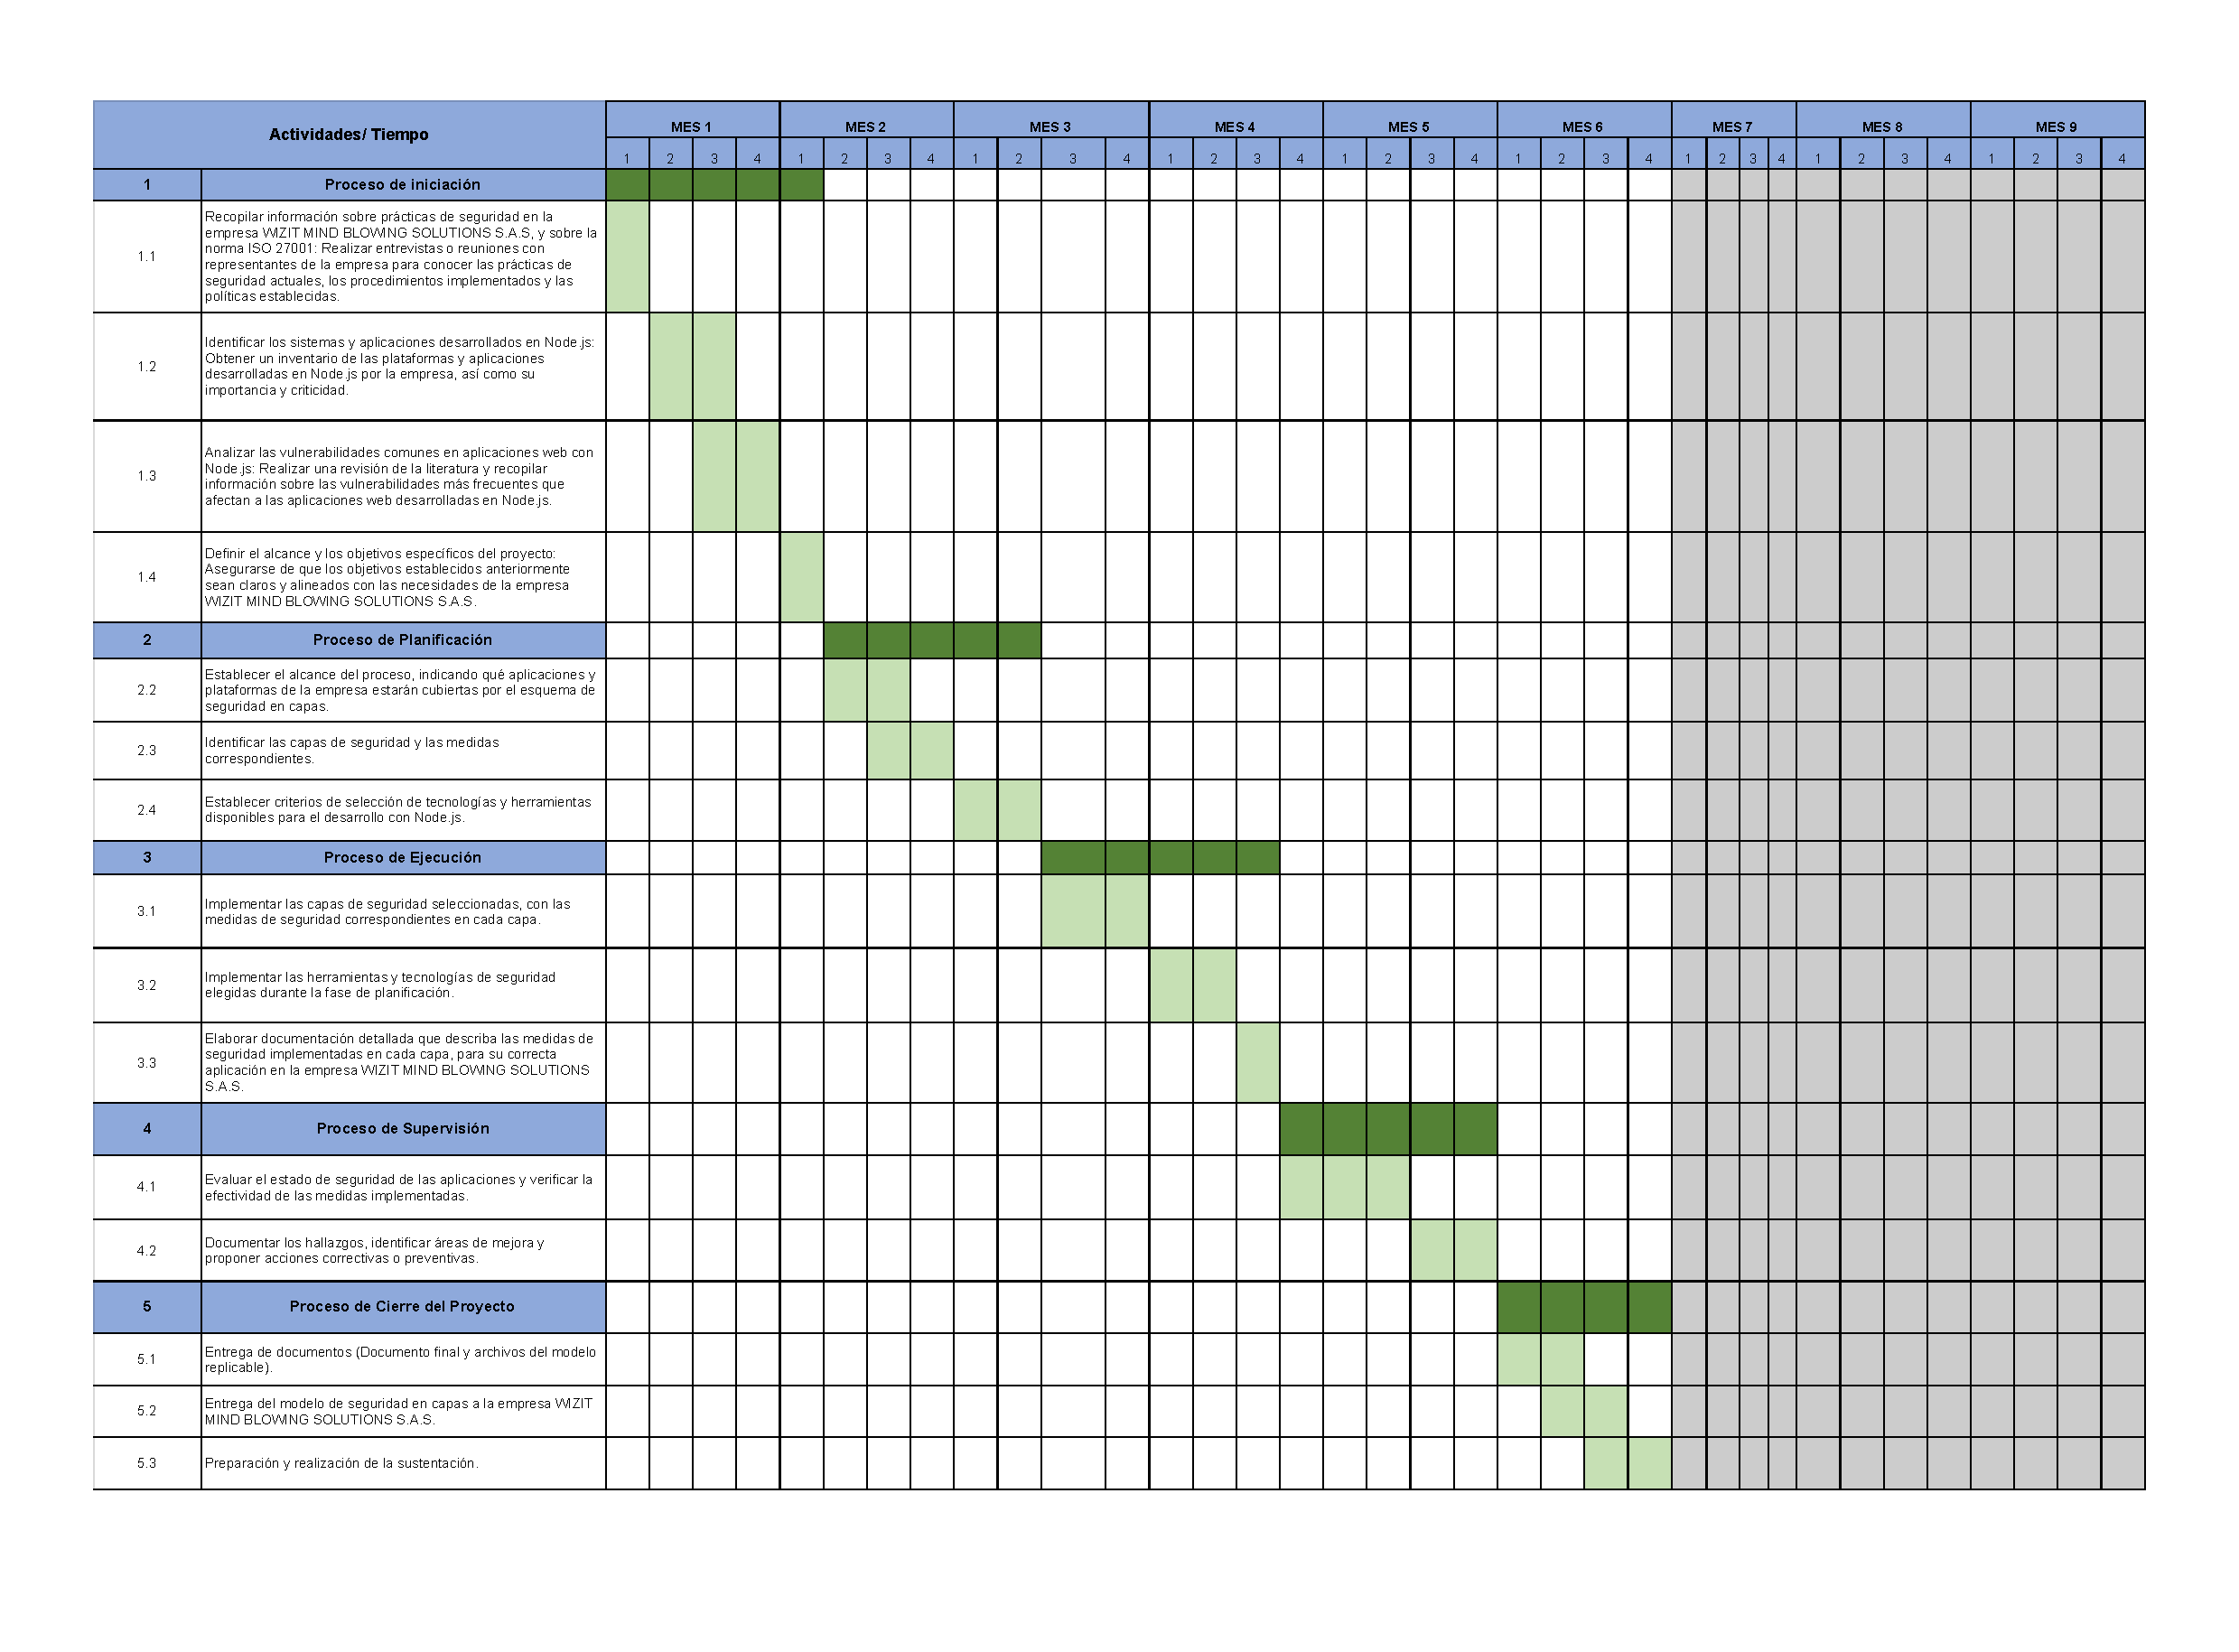
\includepdf[pages=1, scale=0.85, angle=90, offset=1cm 1.5cm, pagecommand={\subsection{CRONOGRAMA}}]{img/Actividades - cronograma.pdf}
\end{landscape}
    \begin{center}
    \item \section{RECURSOS, PRESUPUESTO Y FUENTES DE FINANCIACIÓN}
\end{center}

En la tabla \ref{tab:tbl_recursos} se presenta el presupuesto que se utilizará durante la realización del trabajo de grado para una duración de 9 meses, con base en los criterios de la \textit{Guía de Elaboración de Anteproyectos de Trabajo de Grado - Modalidad Trabajo de Investigación} de la Facultad de Ingeniería Electrónica y Telecomunicaciones de la Universidad del Cauca. Para el cálculo de los valores de los recursos humanos se consideró la última actualización del valor por punto para los empleados públicos docentes, según el decreto 885 del 2 de junio de 2023 y cuyo valor corresponde a \$18,845.00  COP por hora. El presupuesto se planteó de acuerdo con las siguientes características: \par

Director: Msc. Erwin Meza Vega, con disponibilidad de 2 horas semanales durante la realización del proyecto y un reconocimiento de 2,5 puntos la hora. \par

Estudiante: Andrés Felipe Diago Matta, con disponibilidad de 30 horas semanales y un reconocimiento de 1,5 puntos la hora. \ \par

%https://www.funcionpublica.gov.co/eva/gestornormativo/norma.php?i=210811#:~:text=A%20partir%20del%201%20de%20enero%20de%202023%2C%20f%C3%ADjase%20el,pesos%20(%2418.845)%20moneda%20corriente.


\begin{table}[htbp]
  \centering
  \caption{Recursos y presupuesto del trabajo de grado.}
  \begin{tabular}{|c|c|c|c|}
    \hline
    \multicolumn{1}{|c|}{\multirow{2}[4]{*}{\textbf{RECURSOS}}} & \multicolumn{2}{c|}{\textbf{FUENTES}} & \multicolumn{1}{c|}{\multirow{2}[4]{*}{\textbf{TOTAL}}} \bigstrut\\
\cline{2-3}          & \multicolumn{1}{c|}{\textbf{ESTUDIANTES}} & \multicolumn{1}{c|}{\textbf{FIET}} &  \bigstrut\\
    \hline
    \textbf{Director} & \multicolumn{1}{r|}{} & \$3.392.100 & \$3.392.100 \bigstrut\\
    \hline
    \textbf{Co-director} & \multicolumn{1}{r|}{} & \multicolumn{1}{r|}{} & \multicolumn{1}{r|}{} \bigstrut\\
    \hline
    \textbf{Estudiantes} & \$61.057.800 & \multicolumn{1}{r|}{} & \$61.057.800 \bigstrut\\
    \hline
    \multicolumn{4}{|c|}{\textbf{RECURSOS TÉCNICOS}} \bigstrut\\
    \hline
    \multicolumn{4}{|c|}{\textbf{Recursos Hardware}} \bigstrut\\
    \hline
    \textbf{Utilización Equipo} & \multicolumn{1}{r|}{} & \$2.367.504 & \$2.367.504 \bigstrut\\
    \hline
    \textbf{Impresora} & \multicolumn{1}{c|}{\$300.00 } & \multicolumn{1}{r|}{} & \multicolumn{1}{r|}{\$300.00 } \bigstrut\\
    \hline
    \textbf{Otros} & \multicolumn{1}{c|}{\$250.00 } & \multicolumn{1}{r|}{} & \multicolumn{1}{r|}{\$250.00 } \bigstrut\\
    \hline
    \multicolumn{4}{|c|}{\textbf{Recursos Software}} \bigstrut\\
    \hline
    \textbf{OptSim} & \multicolumn{1}{r|}{} & \$3.200.000 & \$3.200.000 \bigstrut\\
    \hline
    \textbf{Matlab} & \multicolumn{1}{r|}{} & \$2.000.000 & \$2.000.000 \bigstrut\\
    \hline
    \multicolumn{4}{|c|}{\textbf{Recursos Bibliográficos}} \bigstrut\\
    \hline
    \textbf{Documentación} & \multicolumn{1}{c|}{\$460.00 } & \multicolumn{1}{r|}{} & \multicolumn{1}{r|}{\$460.00 } \bigstrut\\
    \hline
    \multicolumn{4}{|c|}{\textbf{Recursos Varios}} \bigstrut\\
    \hline
    \textbf{SUBTOTAL} & \$62.067.800 & \$10.959.604 & \$72.567.404 \bigstrut\\
    \hline
    \textbf{AUI (20\%)} & \$12.413.560 & \$2.191.921 & \$14.513.481 \bigstrut\\
    \hline
    \textbf{TOTAL} & \$74.481.360 & \$13.151.525 & \$87.080.885 \bigstrut\\
    \hline
    \end{tabular}%
  \label{tab:tbl_recursos}%
\end{table}%

    \newpage
\begin{center}
\section{CONDICIONES DE ENTREGA}
\end{center}

\begin{itemize}
    \item \textbf{Monografía:} Documento donde se evidencia el trabajo elaborado para alcanzar los objetivos propuestos. Contiene la base conceptual de conocimiento, la descripción detallada del problema, la propuesta y los resultados obtenidos mediante la ejecución del proyecto de grado.
    \item \textbf{Anexos:} Documentación relacionada con el modelo desarrollado, no incluido en la monografía.
    \item \textbf{Artículo:} Documento donde se muestran los resultados y aportes planteados para el trabajo de investigación, en formato IEEE.
    %\item \textbf{Código fuente:} Se compartirán el o los repositorios con el código fuente desarrollado. De esta manera, se tendrá la posibilidad de reproducir las diferentes pruebas y resultados obtenidos.
\end{itemize}
\vspace{0.5cm}
    \printbibliography[title={Bibliografía}]
    %\begin{center}
  \section{REFERENCIAS}
\end{center}

%https://biblioguias.uam.es/citar/estilo_ieee#:~:text=Iniciales%20y%20Apellido%20del%20autor,pp.)%2C%20Mes%20A%C3%B1o.

%\bibliographystyle{bst/IEEEtran} 
%\bibliography{bib/IEEEreferences} 
\begin{thebibliography}{99}

  \bibitem{PedroRuiz} Pedro Alberto Ruiz González, "SEGURIDAD DE APLICACIONES WEB BASADAS EN LAS TECNOLOGÍAS NODE.JS Y MONGODB: ESTUDIO Y CASO DE USO", Universidad Autónoma de Madrid, [Online], Recuperado de: $https://repositorio.uam.es/bitstream/handle/10486/684807/ruiz\_gonzalez\_pedroalberto\_tfm.pdf?sequence=1\&isAllowed=y$

  \bibitem{CarlosSerna} Ortegón Serna, Carlos Andrés, "AMENAZAS, VULNERABILIDADES, FACTORES DE RIESGO Y DEFENSA EN PROFUNDIDAD EN APLICACIONES WEB", Universidad Piloto de Colombia, [Online], Recuperado de: $http://repository.unipiloto.edu.co/bitstream/handle/20.500.12277/4913/00005093.pdf?sequence=1\&isAllowed=y$

  \bibitem{AlexZambrano} Alex Zambrano, Teresa Guarda, Edward Vladimir Haro Valenzuela, Geovanni Ninahualpa Quiña, "Técnicas de mitigación para principales vulnerabilidades de seguridad en aplicaciones web", Universidad de las Fuerzas Armadas ESPE,  Universidad Estatal Península de Santa Elena, Santa Elena, Ecuador – UPSE, Algoritmi Centre, Minho University, Guimarães, Portugal, [Online], Recuperado de: $https://www.researchgate.net/profile/Teresa-Guarda/publication/331178479_Mitigation_techniques_for_security_vulnerabilities_in_web_applications/links/5fabe891a6fdcc331b9478b4/Mitigation-techniques-for-security-vulnerabilities-in-web-applications.pdf$

  \bibitem{AnaSaucedo} Ana Laura Hernández Saucedo, Jezreel Mejia Miranda, "Guía de ataques, vulnerabilidades, técnicas y herramientas para aplicaciones web", Centro de Investigación en Matemáticas (CIMAT) Unidad Zacatecas, , [Online], Recuperado de: $https://www.redalyc.org/pdf/5122/512251501005.pdf$ %2015

  \bibitem{JorgeLascorz} Jorge Martínez Lascorz, "Seguridad web con NodeJS en un sistema de gestión de horarios laborales", UNIVERSIDAD POLITÉCNICA DE MADRID, [Online], Recuperado de: $https://oa.upm.es/48283/8/TFM_JORGE_MARTINEZ_LASCORZ.pdf$ %2017

  \bibitem{DiegoLosada}  Diego Losada Regos, "Seguridad en aplicaciones Web", "Universidad Autónoma de Barcelona", [Online], Recuperado de: $https://openaccess.uoc.edu/bitstream/10609/42542/6/dlosadarTFM0615Memoria.pdf$

  \bibitem{AriasMelo}  Arias Melo Yeison Hernando, "RETOS DE LA SEGURIDAD INFORMÁTICA EN SERVIDORES NODE JS", "Universidad Piloto de Colombia", [Online], Recuperado de: $http://repository.unipiloto.edu.co/bitstream/handle/20.500.12277/2671/Trabajo\%20de\%20grado.pdf?sequence=1\&isAllowed=y$

\end{thebibliography}
    %\bibliographystyle{chicago}
    %\bibliography{biografia}
    \section{ACTA DE PROPIEDAD INTELECTUAL}


%\includepdf[pages={1,2,3}]{img/Acta de propiedad intelectual Firmada - Andres.pdf}

    %\newpage
\section{Anexos}
\subsection{Documentos relacionados con comparación de imágenes}
    \begin{itemize}
    \item El artículo \textbf{Comparison of Geo-Object Based and Pixel-Based Change Detection of Riparian Environments using High Spatial Resolution Multi-Spectral Imagery}  \cite{article23} describe el desarrollo de un sistema de clasificación basado en objetos geográficos para mapear con precisión las clases de cobertura terrestre ribereña para dos imágenes y comparar mapas de cambio derivados de mapas basados en objetos geográficos y por píxel.  Por lo que las técnicas de comparación se realizan de dos diferentes maneras, primero con objetos geográficos como entradas y luego por píxel. Las técnicas de detección de cambios incluyeron la comparación posterior a la clasificación, la diferenciación de imágenes y la transformación Tasseled Cap. Del estudio se concluye que las entradas basadas en objetos geográficos proporcionaron resultados de detección de cambios más precisos que los derivados de las entradas basadas en píxeles, ya que el enfoque basado en objetos geográficos redujo los efectos de sombras y registros erróneos y permitió la inclusión de relaciones de contexto.
    Este documento aporta a nuestro proyecto ya que evidencia la necesidad de una clasificación antes del proceso de comparación porque al clasificar los objetos urbanísticos como las edificaciones se generan unos resultados de detección de cambios más precisos, que si se hace una comparación por píxeles.
    Nuestro trabajo se diferencia de éste, debido a que en este trabajo se quiere analizar los cambios de vegetación a diferencia de nuestro proyecto en donde se requiere analizar cambios urbanos. Adicional a eso se hace el proceso con imágenes Quickbird, las cuales son imágenes satelitales, debido a que no se pueden implementar en el caso de nuestro proyecto ya que hay una limitación tecnológica porque no se disponen de satélites como este en la zona que se quiere analizar, entonces se plantea el proceso con imágenes aéreas provenientes de un dron.
    
    \item El artículo \textbf{Desarrollo de una herramienta de análisis de modificaciones en el terreno mediante el uso de imágenes de drones georreferenciadas o satelitales}  \cite{prostychenko_automatizacion_nodate} describe el desarrollo de un sistema que permite realizar actividades de forma automática correspondientes al proceso de seguimiento de la construcción de infraestructuras de parques fotovoltaicos, implementando para ello herramientas  software como Matlab y LabVIEW que facilitan el seguimiento de la evolución gracias al procesamiento digital de ortofotos geolocalizadas obtenidas mediante drones o alternativamente por satélite, además de la automatización de todo el proceso: adquisición de fotografías y su procesamiento, detección de los distintos elementos del terreno como paneles solares instalados, comparación con resultados anteriores y planos técnicos, obtención de resultados de avance y generación de informes.
    Este documento aporta a nuestro proyecto en la implementación y desarrollo de herramientas que permitan la realización de un proceso completo de detección de modificaciones entre imágenes de manera automática, desde la adquisición de fotografías y su procesamiento, detección de los distintos elementos del terreno, además de comparación con resultados anteriores y planos técnicos, que permiten obtención de resultados de avance y generación de informes. Por otra parte, se centran en el análisis y seguimiento de la construcción de infraestructuras de parques fotovoltaicos, alejándose de nuestro centro de estudio que correspondiente a la zona de construcción urbana, además de tomar en consideración análisis con imágenes satelitales, las cuales no están previstas dentro de nuestro proyecto por factores de tiempo y costos.
    \item El artículo \textbf{Monitoring of urban growth in the state of Hidalgo using Landsat images}\cite{LeautaudValenzuela2017} Se realiza el análisis de una técnica para la detección de plaga forestal mediante fotografías aéreas infrarrojas.  La utilización de fotografías aéreas digitales en color e infrarrojo permitió obtener imágenes VIR (visible + infrarrojo) con 4 bandas y una resolución aproximada de un metro por píxel. Las principales repercusiones en las áreas a evaluar tienen relación con las políticas de desempeño forestal, que no siguen el funcionamiento (incluido el saneamiento) en el área. Las fotografías aéreas digitales son útiles para la detección de árboles afectados en los bosques por medio de la interpretación visual con una eficiencia del 98 por ciento. 
    El proyecto contribuye con la demostración de técnica de detección de daños en el área seleccionada, que podría ser adaptado en este caso para cambios en estructuras, esta detección se realiza mediante el análisis de imágenes con uso de tecnología infrarroja, que corresponde a un aporte a resaltar por la seguridad en los resultados y una facilidad relativa en el proceso de revisión de los mismos que puede ser un proceso extenso con imágenes satelitales.
    Se difiere principalmente en las técnicas propuestas a usar para la comparación de las imágenes, el adaptar la tecnología de detección descrita en el artículo implicaría un cambio significativo en el proceso que se desea llevar con el análisis de las imágenes tomadas por drones, teniendo en cuenta que las plataformas software que ofrecen imágenes satelitales no reciben una actualización constante en el área a la que esta dirigida el proyecto, obstaculizando los periodos de tiempo deseados para la comparación de imágenes.
    \end{itemize}
\subsection{Documentos relacionados con control urbano}
 \begin{itemize}
        \item El artículo \textbf{Satellite monitoring of urbanization and environmental impacts—A comparison of Stockholm and Shanghai }\cite{HAAS2015138} plantea el monitoreo del crecimiento urbano a partir de imágenes satelitales, con el fin de ver el impacto que tiene el cambio de uso de la tierra en el medio ambiente, para ello se usan técnicas de análisis de imágenes como el análisis de texturas mediante la matriz de co-ocurrencia de nivel gris (GLCM) el cual mide las variaciones locales en la matriz de coocurrencia de nivel gris, esto con el fin de generar una clasificación de los mapas de uso del suelo y cobertura del suelo (LULC), posteriormente se usa una Máquina de Vector Soporte para clasificar las diferentes zonas entre agricultura, bosque, agua (humedales y acuicultura).
        Este artículo aporta a nuestro proyecto el uso de la Máquina Vector ya que este método puede clasificar las edificaciones de otros elementos del paisaje urbano como carreteras, parques entre otros, que son zonas que no se desean procesar para realizar la comparación lo que haría un sistema más eficiente ya que no se comparan elementos innecesarios.
        La principal diferencia entre este trabajo y el nuestro es que no se genera una comparación píxel a píxel que permita la identificación exacta de los píxeles que cambian con respecto a la imagen anterior, o una comparación por objetos obtenido de la clasificación previa, sino que se genera una comparación global de las zonas duras actuales. En nuestro trabajo se requiere hacer una comparación píxel a píxel o por objetos para poder identificar la ubicación de la edificación que está presentando novedades.
        
        \item El artículo \textbf{A systematic review and assessment of algorithms to detect, characterize, and monitor urban land change}\cite{REBA2020111739} hace una revisión y evaluación sistemática de algoritmos para detectar, caracterizar y monitorear el cambio de suelo urbano, para dar a conocer la gran variedad de métodos disponibles en este campo.  En este artículo se especifica claramente las etapas por las que pasan las imágenes para generar la detección de cambios urbanos generales, las cuales son: el preprocesamiento de imágenes, la comparación de imágenes, que normalmente ocurre usando un operador de razón, razón logarítmica o razón basada en vecindad y el umbral del indicador de cambio de imagen.
        
        Este artículo aporta a nuestro proyecto una visión general de las técnicas usadas en diferentes estudios para el monitoreo urbano, organizándolo en diferentes etapas, de las cuales se resalta las de control los cuales se refieren al cambio de cobertura terrestre, en donde se identifica que el método de transformación mencionado se puede adaptar a la comparación que se necesita en el trabajo propuesto ya que este método se basa en el cálculo de vectores de diferencia entre unidades de análisis dadas tanto la magnitud como la dirección del cambio.
        Nuestro trabajo se diferencia de los documentos vistos en la revisión sistemática plasmada en este documento ya que, se necesita una comparación de cada uno de los puntos de la imagen y no una comparación general que es lo que se hace para ver el impacto de la urbanización con los años, además, en este documento no se considera el procesamiento previo de imágenes ni los pasos de evaluación de la precisión, procesos indispensables para realizar el procesamiento de las imágenes. Por otro lado, se plantea que los estudios realizados en el monitoreo de los cambios urbanos se realizan principalmente en países desarrollados que tienen ingresos altos como China y Estados Unidos por lo que se encuentra una brecha en países como Colombia. Finalmente se destaca la necesidad de más estudios que distinguen la variación intraurbana ya que los estudios actuales se limitan a ver el crecimiento urbanístico, pero no lo que está sucediendo al interior de las ciudades, factor que se quiere abarcar con nuestro trabajo.
        
        \item El artículo \textbf{Safety Challenges for Integrating U-Space in Urban Environments}\cite{9476883} presenta el proyecto desarrolado en Europa de la iniciativa U-space para permitir la integración de miles de drones en los cielos . El análisis concluye que el marco actual no es lo suficientemente maduro para abordar algunos de los desafíos emergentes identificados. El trabajo futuro debería incluir el uso de técnicas de ingeniería de resiliencia para mitigar los riesgos vinculados a los sistemas autónomos y un uso equilibrado de la Inteligencia Artificial, cuyos beneficios a medio / largo plazo superará los retos iniciales de seguridad.
        En el artículo se pueden conocer y relacionar los retos que implican el uso de red de drones para la obtención de imágenes satelitales en espacios urbanos, con técnicas presentadas en el marco regulador de la gestión del tránsito aéreo, dichos desafíos pueden ser tenidos en cuenta en el momento de diseño de recorrido y distribución de los drones que se pretenden implementar en la parte de hardware. Se propone técnicas de ingeniería de resiliencia para buscar la solución estos, con uso de sistemas autónomos acoplados con Inteligencia Artificial.
        El proyecto se centra en las implicaciones y procesos necesarios en el control de despliegue de una red de drones en áreas urbanas, sin tomar plantear un sistema que permita analizar las diferencias en imágenes obtenidas por los drones para tener en cuenta esos cambios interurbanos.
        
        \item El artículo \textbf{Análisis de la minería mediante la generación de cartografía
        por medio de drones (UAV) como implementación de análisis de riesgos en el Municipio de Une Cundinamarca}\cite{rojas_velasquez_alisis_nodate} propone un sistema de actualización de información cartográfico (POT, PBOT o EOT) a partir del uso de nuevas tecnologías como los drones para la toma de imágenes puesto que, permiten reducir el gasto de tiempo en este tipo de estudios, además de facilitar la accesibilidad a ciertos tipo de terrenos. El estudio que aquí se abarca se enfoca principalmente en las áreas de explotación minera para definir los componentes de riesgo que conlleva el desarrollo de esta actividad en el terreno, su desarrollo se enfoca en la toma de imágenes aéreas y su respectivo procesamiento.
        Aporta a nuestro proyecto desde la exposición de la falta de control en el esquema y plan de ordenamiento territorial del país y como este se ha ido deteriorando con el paso del tiempo, proponiendo una solución basada en la inclusión de tecnología que representan los UAV en temas relacionados a cartografía que permitan contribuir a actualizaciones de los instrumentos técnicos de urbanización como el POT, PBOT o EOT de los municipios. 
        A diferencia del nuestro, en este documento el centro de estudio está en los municipios de la zona rural ya que son las zonas de riesgo afectadas por el área de reserva minera, implicando brechas en cuanto a los resultados esperados en comparación a nuestro proyecto ya que, las características del suelo y parámetros de comparación a tener en cuenta en el procesamiento de imágenes resultan diferentes a los de la zona urbana en este caso el centro histórico de la ciudad de Popayán en donde se desea desarrollar nuestro proyecto.
        
        \item El artículo \textbf{Uso de la tecnología UAV en el marco de un proyecto urbanístico de escala media con fines de ordenamiento territorial} \cite{garcilar_lallana_uso_2019} plantea una comparación de la eficiencia de los métodos tradicionales y la implementación de nuevas tecnologías para la regulación del control urbano (ordenamiento territorial), a partir de la comparación entre terrenos, específicamente entre la superficie y perímetro obtenida a partir de un relevamiento de la zona y  el plano antecedente del mismo, a través de vuelos fotogramétricos con UAV y la utilización de subproductos, validando las condiciones necesarias que deberían presentar los terrenos y alrededores con el fin de definir la  mensura urbana del mismo.
        Este documento aporta a nuestro proyecto parámetros para tener en consideración durante la etapa de comparación de terrenos, con fines de control territorial,  ya que se toma en cuenta factores como la superficie y perímetro de los mismos, a partir, de un relevamiento realizado en la zona a través de vuelos fotogramétricos con UAV, adicionalmente nos da a conocer algunas retos a los que nos tendremos que enfrentar en cuanto a la información que nos brinde la institución pública en este caso la curaduría urbana, ya que algunos predios pueden no presentar planos antecedentes y por ende no se pueda hacer posible la comparación con el relevamiento realizado.
        A diferencia del nuestro, el proyecto centra gran parte de su desarrollo al control y procesamiento posicional del vuelo fotogramétrico, el cual no cumple con el interés de nuestro proyecto, adicional a esto, no se abarca desarrollo ni implementación de algún prototipo tecnológico, ya que todas las herramientas utilizadas son softwares existentes en el mercado. De igual manera, no se exponen acciones de notificación ante los predios que presentaron cambios en contra de la norma establecida.
        
        \item El artículo \textbf{Using unmanned aerial systems (UAS) for remotely sensing physical disorder in neighborhoods }\cite{grubesic_using_2018}  realiza un analisis del entorno ecologico de una localidad a través de la recolección de imágenes captadas por drones que permiten identificar detalles del desorden urbano para lograr analizar el comportamiento de los habitantes y el uso de espacios públicos y como estos factores inciden en la salud, criminalidad o cultura del lugar.
        Aporta a nuestro proyecto desde el análisis sobre las ventajas que tienen los UAS frente a otros métodos de recolección de información a través de imágenes en cuestión de calidad y detalles que se pueden obtener. aportando una visión general de las ventajas que nos puede traer el uso de drones. 
        El trabajo realizado en esta investigación se enfocaba en estudiar en las imágenes recolectadas el desorden físico evidenciado en terrenos o edificios abandonados, grafitis, lugares donde la gente deposita su basura, entre otros, con el objetivo de realizar un análisis del contexto del área analizada y como este puede influir en la salud de los habitantes, en como disfrutan los espacios públicos y en la criminalidad de la zona, alejándose del objetivo de nuestro proyecto.
        \end{itemize}
\subsection{Documentos relacionados con toma de imágenes aéreas}
 \begin{itemize}
        \item El artículo \textbf{Improvement of Workflow for Topographic Surveys in Long Highwalls of Open Pit Mines with an Unmanned Aerial Vehicle and Structure from Motion}  \cite{rs13173353} plantea la realización de levantamientos topográficos en minas activas es un desafío debido a las operaciones continuas y los peligros en muros altos. Se realizan vuelos con drones en busca de la mejor configuración en términos de modo de altitud y ángulo de cámara, para producir una representación digital de topografías utilizando Structure from Motion. El estudio se llevó a cabo en una mina de caolín activa cerca del Parque Natural del Alto Tajo del Centro-Este de España. Se demostró que un modo de vuelo de dron de fachada combinado con un ángulo de cámara nadir, y programado automáticamente con un software de planificación de misiones basado en computadora, proporciona las topografías más precisas y detalladas, en el menor tiempo y con mayor seguridad de vuelo. Estas topografías permitieron la detección de un 93,5 por ciento más de discontinuidades que los levantamientos por encima del nivel medio del mar, el enfoque común utilizado en las áreas mineras. 
        
        Es posible adaptar del artículo, cuya base es el uso de drones con la tecnología Structure from Motion para identificar falencias en áreas específicas, las técnicas descritas. Se tiene una descripción del acomodamiento de parámetros de la cámara de los drones, posición y ángulo para la obtención de imágenes óptimas para un análisis mejor de las mismas. Se diferencia ya que el objetivo de análisis de área que se realiza a partir de las fotografías obtenidas por los drones difiere al proceso que se quiere ampliar en el anteproyecto, pues este tiene relación con el cambio de estructuras en un área urbana en este anteproyecto, por lo que no se hace un énfasis en características físicas del área, sino en cambios que buscan ser detectados. Además del uso de una red amplia de drones, que en este caso no es necesaria pues se quiere abarcar como espacio el centro de Popayán, lo que no implicaría el uso de numerosos drones.
        
        \item El artículo \textbf{Generación de cartografía catastral urbana comparativa, mediante la utilización de geo-tecnologías con fines de ordenamiento territorial en la ciudad de Bolívar, cantón Bolívar, provincia del  Carchi} \cite{carrera_herrera_generacion_2018}  plantea el uso de vehículos no tripulados y GPS diferencial para realizar imágenes aéreas de la ciudad Bolívar con el fin de proponer un plan de ordenamiento territorial para la zona, entendiendo la dinámica de crecimiento que tiene actualmente la ciudad. Además, se realiza un análisis de cobertura de servicios y el uso del suelo actual.
        
        Este artículo aporta a nuestro proyecto una visión general de las En este articulo aporta a nuestro mediante la descripción del método utilizado para realizar el vuelo fotogramétrico digital realizado a una escala de 1:100 con GSD 6cm. Además, describe se describen los errores de exactitud que puede ser por omisión, consistencia lógica o exactitud temática respecto a la representación gráfica de los elementos a cartografiar.
        A pesar de utilizar el mismo medio para obtener las imágenes aéreas del territorio, en este caso la metodología se basa en la toma de imágenes, abstracción de datos, comparación con la referencia existente y proposición de modelos de orden territorial que permitan un buen crecimiento de la ciudad, por ende, no existe más de una toma de datos o la necesidad de una amplia base de datos para almacenar la información. Por otra parte, en este proyecto se basa en una zona mayormente agraria y para la toma de datos bastaba con captar la utilización del suelo, pero no detalles de las edificaciones como se necesita en nuestro proyecto.
        
        \item El artículo \textbf{Aplicación de fotogrametría con dron para la actualización de los factores físicos del catastro urbano del distrito de Ticapampa } \cite{morales_alvarado_aplicacion_2021}  muestra los resultados de una investigación realizada acerca del uso de fotogrametría con dron para actualizar los factores físicos del catastro en Ticapampa sustentar la planificación urbana y de servicios.
       Este artículo aporta a nuestro proyecto ya que durante el desarrollo del trabajo se describen todas las características y especificaciones utilizadas para la recolección de imágenes por medio de drones, enfocándose en el reconocimiento de características físicas generales de un área geográfica especifica, asemejándose en ese aspecto al objetivo de nuestro proyecto. 
        El objetivo de este proyecto se basa en obtener una actualización de los datos territoriales que no han sido actualizados por más de 50 años en el territorio seleccionado, por ende, no es necesario realizar más de una toma de imágenes como se plantea en nuestro proyecto para poder comparar datos actualizados que permitan la notificación de cambios recientes y un control de nuevas construcciones
        \end{itemize}

\end{document}
